\section{Implementation}
\label{sec:impl}

We were able to extend Bud to support \lang with relatively minor changes. Bud
initially had about 7200 lines of code (LOC). Supporting the core lattice
features (the \texttt{Bud::Lattice} base class and the mapping from identifiers
to lattice values) required about 300 LOC. The builtin lattice classes
constituted an additional 300 LOC. Modifying Bud's fixpoint logic to include
lattices required only 10 LOC, while the program rewriting required to enable
seminaive evaluation required 100 LOC. Modifying Bud's collection classes to
merge together embedded lattice values required modifying about 125 LOC. Along
with other miscellaneous changes, adding support for \lang required less than
900 new lines of code. This experience suggests that support for lattices can be
added to an existing Datalog engine in a relatively straightforward manner.

\subsection{Evaluation strategy}
\nrc{TODO: describe how we generalize seminaive to \lang, justify why it is correct.}

\subsection{Performance validation}
\label{sec:lattice-perf}

\begin{figure}[t]
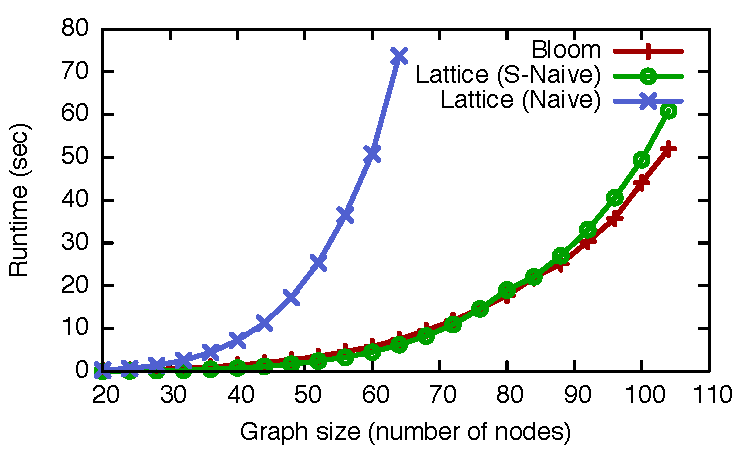
\includegraphics[width=\linewidth]{fig/sn_perf}
\caption{Performance comparison of three different methods for computing the
  transitive closure of a graph.}
\label{fig:tc-perf-graph}
\end{figure}

To validate the effectiveness of semi-naive evaluation for \lang programs, we
wrote two versions of a program to compute the transitive closure of a directed
acyclic graph. One version was written in Bloom and used traditional
set-oriented collections. The other version was written in \lang and used
morphisms over the \texttt{lset} lattice. For the \lang version, we ran the
program both with and without semi-naive evaluation enabled. As input, we used
on synthetic graphs of various sizes---in a graph with $n$ nodes, each node had
$O(\log_2 n)$ outgoing edges. We ran the experiment on a late 2010
MacBook Air with a 2.13 Ghz Intel Core 2 Duo processor and 4GB of RAM, running
Mac OS X 10.7.3 and Ruby 1.8.7-p352. We ran each program variant five times on
each graph and report the mean elapsed wall-clock time.

Figure~\ref{fig:tc-perf-graph} shows how the runtime of each program varied with
the size of the graph. Note that we only report results for the naive \lang
strategy on small input sizes because this variant ran very slowly as the graph
size increased. The poor performance of naive evaluation is not surprising:
after deriving all paths of length $n$, naive evaluation will then rederive all
those paths at every subsequent ``step'' of the fixpoint computation. In
contrast, after computing length $n$ paths, a semi-naive strategy will only
generate length $n+1$ paths in the next step. Bloom and semi-naive \lang achieve
similar results. We instrumented Bud to count the number of derivations made by
the Bloom and seminaive lattice variants---as expected, both programs made about
the same number of derivations. These results suggest that our implementation of
semi-naive evaluation for \lang is effective and performs comparably with a
traditional Datalog system.

For large inputs, Bloom begins to outperform the seminaive lattice variant. This
is because the current lattice implementation copies more data: lattices are
immutable, so the \texttt{lset} merge function allocates a new set to hold the
result of the merge. In contrast, Bloom collections are modified in-place.
